\documentclass{article}
\usepackage{amsmath, graphicx, float, blindtext} % for dummy text
\graphicspath{ {./images/} }
\title{Chapter 9: Hierachical Models}
\author{Shubham Gupta}
\begin{document}    
\maketitle

\section{Introduction}

\begin{itemize}
    \item They involve multiple parameters.
    \item When the value of one parameter $\theta$ depends on another variable  $\omega$, the hierachical structure of these variables can be represented by a hierachical model.
    \item To infer these parameters, we apply the joint probability rule for the parameters. \[
            P(\theta, \omega|D) \propto P(D|\theta, \omega) p(\theta, \omega) 
        .\] 
        \[
            = P(D|\theta) * P(\theta|\omega) * P(\omega)
        .\] 
    \item The above equation implies that value of $D$ is dependent only on  $\theta$ and independant of other variables. Similarly, the value of  $\theta$ is dependant only on the value of  $\omega$ and is conditionally independant of all other parameters.
    \item The dependencies between parameters are useful because:
        \begin{itemize}
            \item They are meaningful for the given application
            \item Because of dependencies across parameters, they can jointly inform all parameter estimates.
            \item Easier convergence with smart algorithms that exploit this joint probability.
        \end{itemize}
\end{itemize}

\subsection{Coin flipping from a single mint}

\begin{itemize}
    \item We will use bernoulli distribution for the data and beta distribution for the prior. \[
            y_{i} \approx dbern(\theta) 
        .\] 
        \[
            \theta \approx dbeta(a, b)
        .\] 
    \item We know that $a$ and $b$ can be represented as using mode $\omega$ and concertration $\kappa$ as:
        \[
            a = \omega(\kappa-2)+1 
        .\] 
        \[
            b = (1-\omega)(\kappa - 2) + 1 
        .\] 
    \item Hence, we can write $\theta$ as:
        \[
            \theta \approx dbeta(\omega(\kappa-2)+1, (1-\omega)(\kappa - 2) + 1)
        .\] 
        \begin{itemize}
            \item The value $\kappa$ controls how close the value of  $\omega$ is  $\theta$.
            \item Higher value of $\kappa$ = Closer to value of $\theta$
        \end{itemize}
    \item Let us assume $\omega$ is another parameter to be estimated. Assume this to be a beta distribution: $\omega \approx beta(\omega | A_{\omega}, B{_\omega})$
    \item We know the value of $\omega$ is closer to the mode of the distribution in this case i.e: $\frac{A_{\omega}-1}{A_{\omega}+B_{\omega}-2}$
    \item Substituting bayes rule, we get:
        \[
            p(\theta, \omega | y) = \frac{p(y | \theta, \omega) p(\theta, \omega)}{p(y)}            
            = \frac{p(y|\theta)p(\theta|\omega)p(\omega)}{p(y)}
        .\] 
    \item We have the equations for all of the above components. We can get the posterior probability by solving the above equation.
    \item We can solve them using grid approximation as well as the parameters are finite. 
\end{itemize}

\subsection{Multiple coins from single mint} 
\begin{itemize}
    \item Assume we have multiple coins for a single mint. Each coin will now have it's own parameter $\theta_{s}$ and we will estimate this using all the data for $\omega$. 
\end{itemize}

\subsection{Real example}
\begin{itemize}
    \item For the multiple coins problem, we do not know the value for $\omega$ in advance. We will have to estimate it from the data available.
    \item We will assume $\omega$ follows a gamma distribution. The gamma distribution has the following formula: $gamma(\kappa|s, r)$. Here, $s$ is the shape parameter and $r$ is the rate parameter. 
    \item We will use the parameters $s$ =1.56 and $r$ =0.0312 because these values have a boundary at 0 and infinite possible positive values.  
    \item 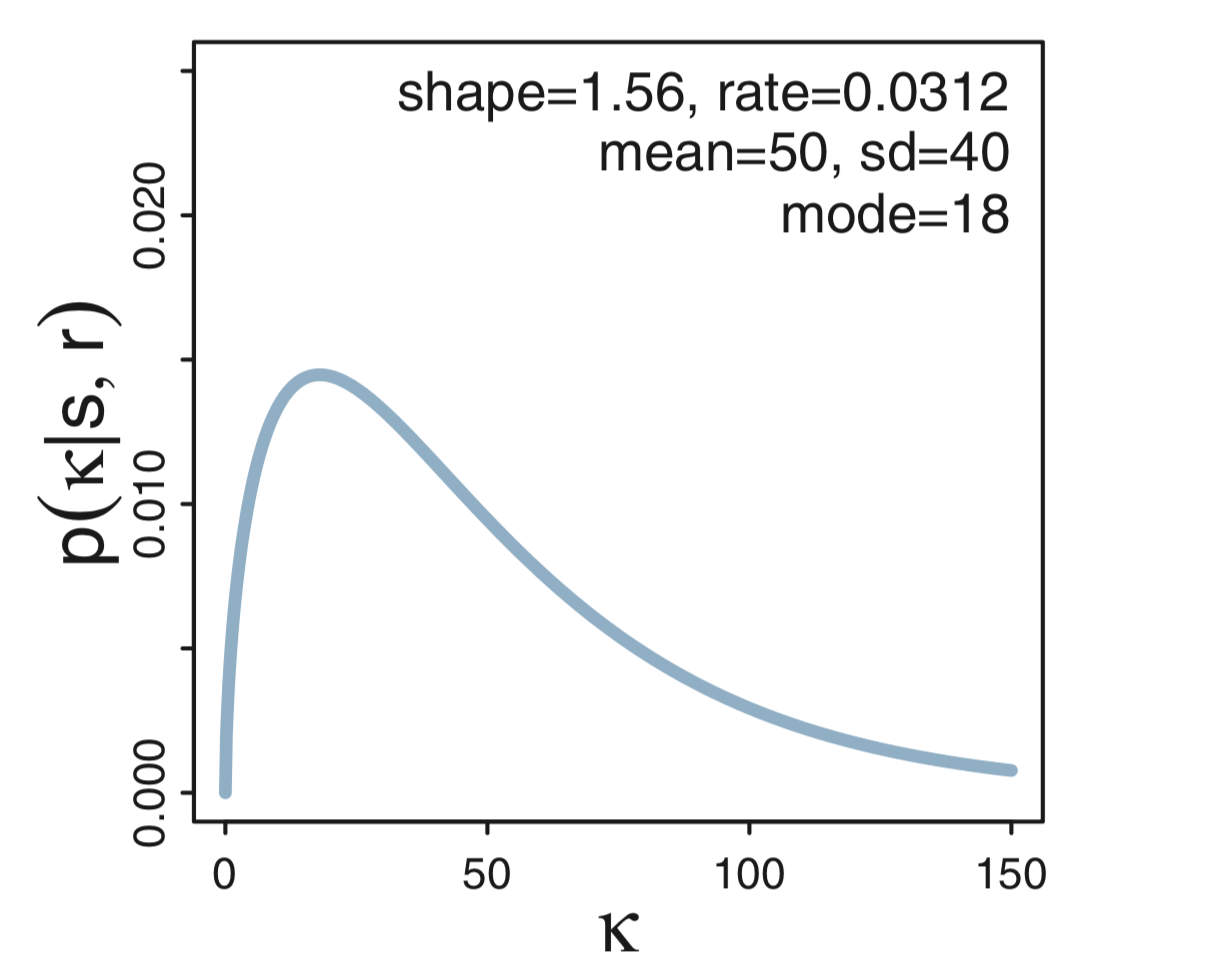
\includegraphics[scale=0.3]{gamma_distribution}
    \item Mean: $\mu = \frac{s}{r}$ 
    \item Mode: $\omega = \frac{s-1}{r}$
    \item SDev: $\sigma = \frac{\sqrt{s}}{r}$
    \item We can derive $s$ and $r$ from the above as:
        \[
            s = \frac{\mu^2}{\sigma^2} 
        .\] 
        \[
            r = \frac{\mu}{\sigma^2}
        .\] 
        when the mean $\mu \textgreater 0$
    \item It can also be written as:
        \[
            s = 1 + \omega r
        .\] 
        \[
            r = \frac{\omega + \sqrt{\omega^2 + 4\sigma^2}}{2\sigma^2} 
        .\] 
        \begin{figure}[H]
            \centering
            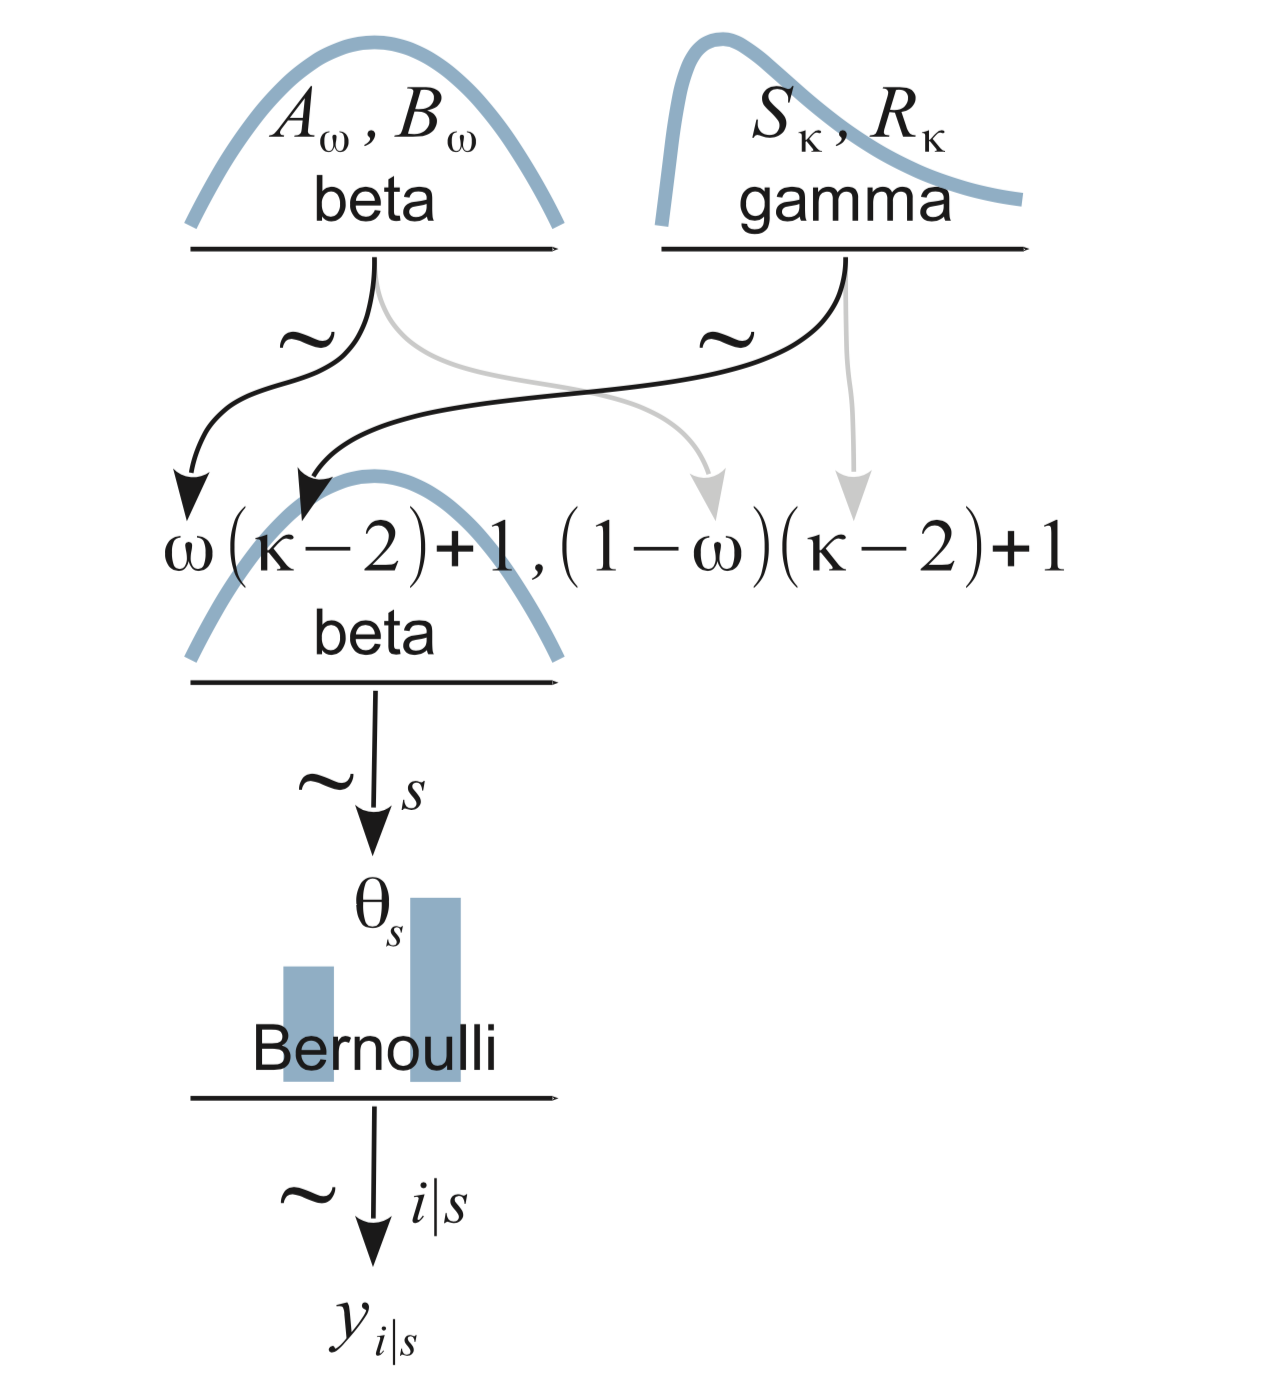
\includegraphics[width=0.5\textwidth]{model}
            \caption{Hierachical Model}
            \label{fig:}
        \end{figure} 
\end{itemize}
\subsection{Theraupeutic Touch}
\begin{itemize}
    \item Relieve congestion and improve balance by manipulating "energy field" without touching the patient.
    \item Experiment
        \begin{itemize}
            \item Practitioner should be able to tell if hand is near their hand without touching the hand.
            \item Experimenter flips a coin. Depending on the outcome, places hand above or below practitioner hand.
            \item Practitioner guesses if hand is above or below.
            \item Chance performance for guessing the result is 0.5
        \end{itemize}
    \item Questions:
        \begin{itemize}
            \item How much did group differ from chance performance?
            \item How much did each individual differ from chance performance?
        \end{itemize}
\end{itemize}
\section{Shrinkage}
\begin{itemize}
    \item Estimates of low-level params are pulled together than they would if they were higher-level params. This pulling is called \textbf{shrinkage}.
    \item It occurs because:
        \begin{itemize}
            \item Subset of data is directly dependant on the low-level parameter.
            \item The higher-level params that depend on the low-level params.
        \end{itemize}
    \item Shrikage occurs because of hierachical models, not bayesian estimation.
    \item Intuitively, shrinkage occurs because data from all individuals influence the higher-order params, and these params in-turn influence the estimates for each individual.
\end{itemize}
\section{Extending the hierachy}
\begin{itemize}
    \item We can model problems as hierachical models of multiple levels.
    \item Baseball players
        \begin{itemize}
            \item They bat. Sometimes they get a hit. 
            \item Different positions for each player. Categorize by player positions.
            \item Hence, we can estimate abilities for each player AND each position.
        \end{itemize}
        \begin{figure}[H]
            \centering
            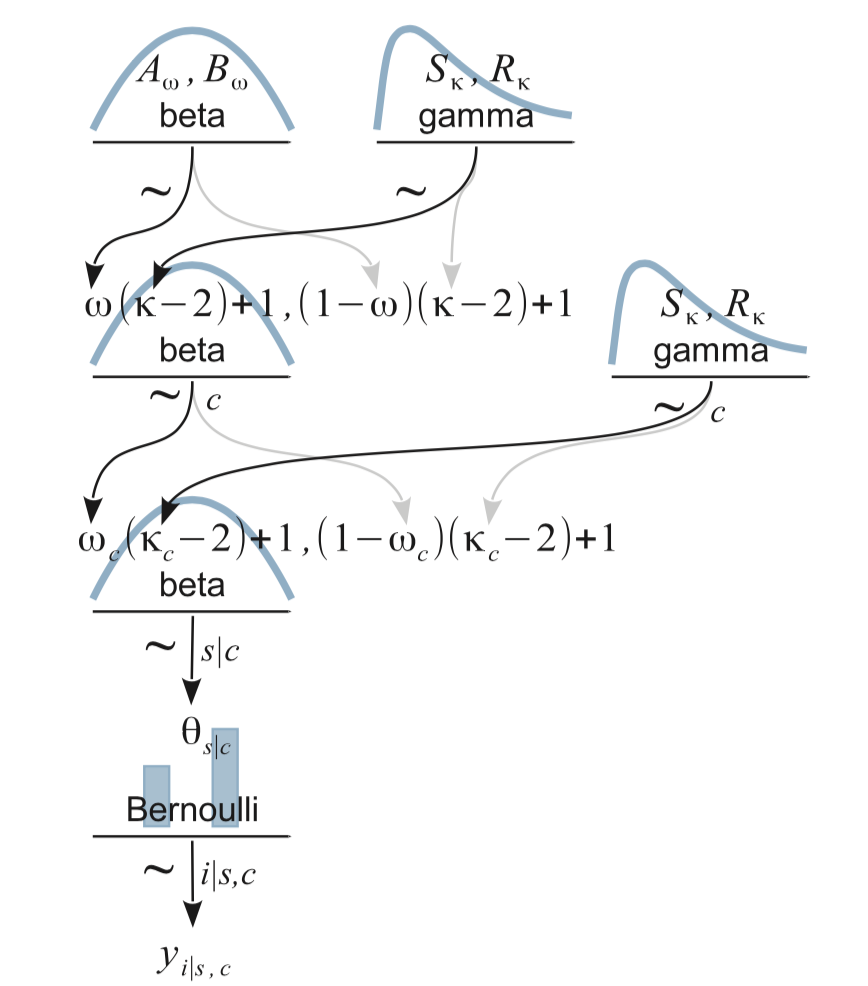
\includegraphics[width=0.3\textwidth]{baseball_model}
            \caption{Baseball Hierachical model}
            \label{fig:}
        \end{figure}
        \begin{itemize}
            \item Each player is denoted by $s$.
            \item Number of oppourtunities to bat: $N_{s|c}$.
            \item Number of hits: $z_{s|c}$
            \item Primary position of a player:  $c_{s}$
        \end{itemize}
\end{itemize}
\section{NCSU Hierachical models}
\begin{itemize}
    \item Presentation is available here: https://www4.stat.ncsu.edu/~reich/ABA/notes/Hier.pdf.
    \item Hierachical models are similar to divide and conquer problems. 
    \item They are simple to implement because of MCMC.
    \item There are 3 main layers bayesian modelling:
        \begin{itemize}
            \item Data Layer: $[Y| \theta, \alpha]$ is the likelihood of the data $Y$.
            \item Process Layer: $[\theta | \alpha]$ is the model for parameters $\theta$ that define latent data generation process.
            \item Prior Layer: $\alpha$ define the prior for the hyperparameters.
        \end{itemize}
        \subsection{Data Layer}
        \begin{itemize}
            \item $S_{t} \implies$ susceptable individuals
            \item $I_{t} \implies$ infected individuals at time $t$.
            \item $Y_{t}$ is the number of observed cases at time $t$.
            \item Data layer models our ability to process $I_{t}$.
            \item NO false positives and false negative probability of $p$.
        \end{itemize}
        \subsection{Process Layer}
        \begin{itemize}
            \item Scientific understanding of the disease is used to model how it will spread.
            \item We will use the Reed-Forest model
                \[
                    I_{t+1} \sim Binomial[S_{t}, 1 - (1 - q)^{I_{t}}] 
                .\] 
                \[
                    S_{t+1} = S_{t} - I_{t+1}
                .\]  
            \item This model assumes that all the infected individuals at time $t$ are removed before time $t+1$
            \item $q$ is probability of non infected person coming in contact with infected person and getting the disease.
        \end{itemize}
        \subsection{Prior Layer}
        \begin{itemize}
            \item The process layer expresses disease dynamics up to a few unknown parameters.
            \item These unknown parameters are the priors
            \item Prior Layer:
                \[
                    I_{t} \sim  Poisson(\lambda_{1})
                .\] 
                \[
                    S_{t} \sim Poisson(\lambda_{2})
                .\] 
                \[
                    p, q \sim beta(a,b) 
                .\] 
        \end{itemize}
        \begin{figure}[H]
            \centering
            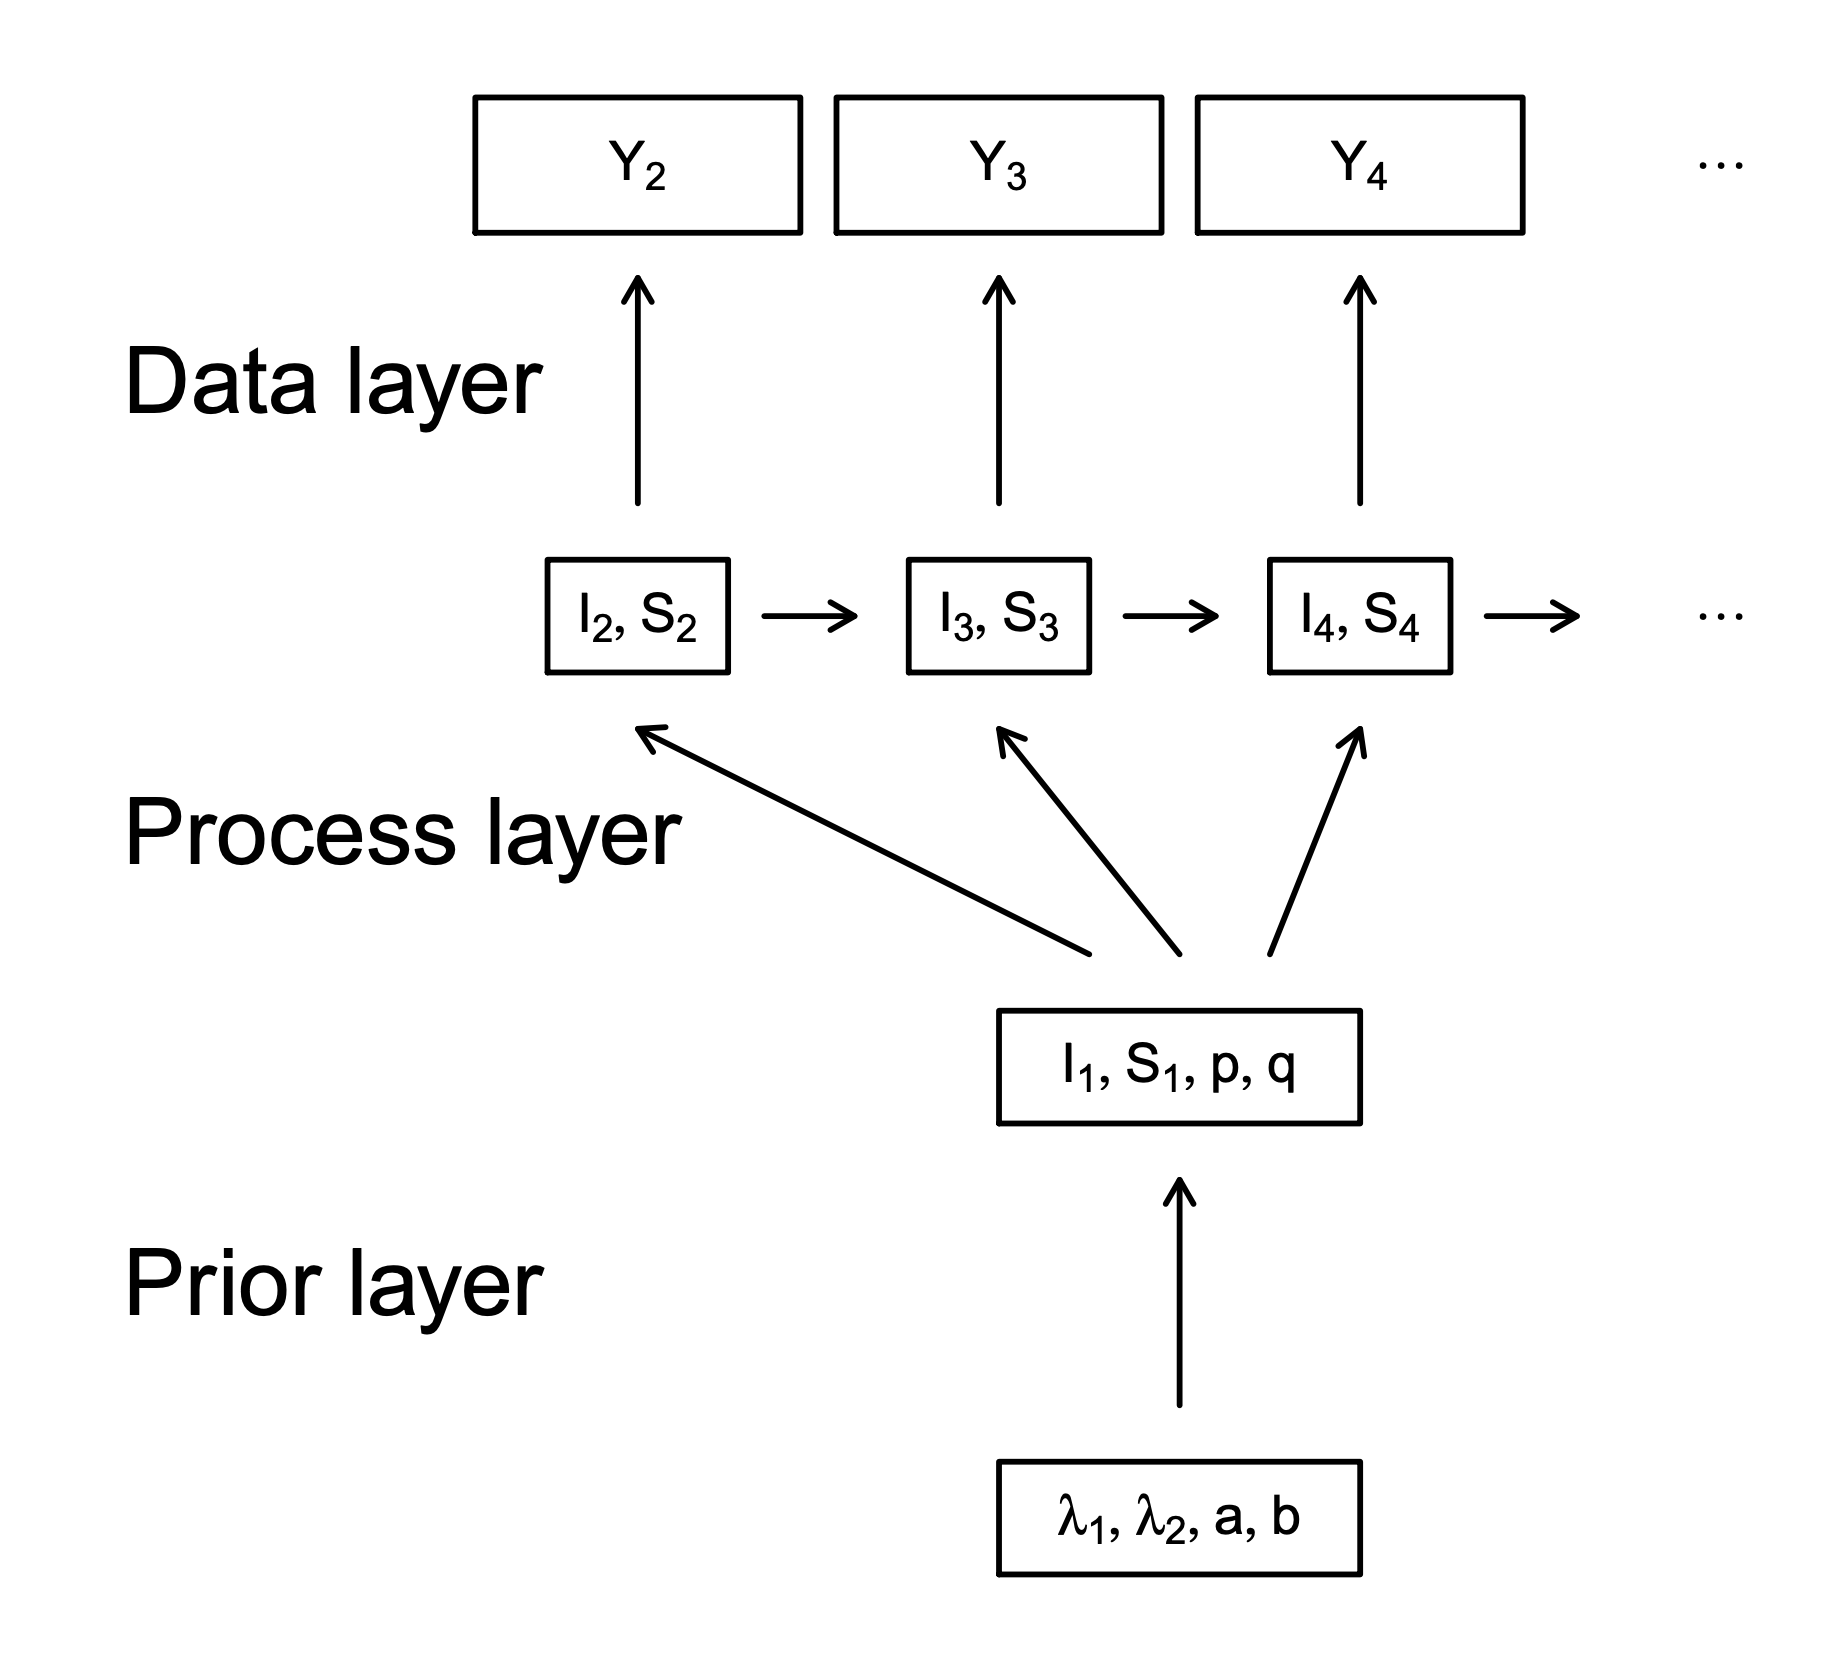
\includegraphics[width=0.8\textwidth]{dag}
            \caption{DAG}
            \label{fig:dag}
        \end{figure}
        \subsection{Hierachical models and MCMC}
        \begin{itemize}
            \item MCMC is efficient for hierachical models with even larger number of parameters.
            \item Only consider "connected" nodes when we update each parameter.
                \[
                    1. [\theta_{i}|.]
                .\]
                \[
                    2. [\mu|.]
                .\] 
                \[
                    3. [\sigma^2|.]
                .\] 
                \[
                    4. [\tau^2|.]
                .\] 
            \item Each of the above updates is drawn from a 1-D normal or inverse gamma distribution. 
            \item Didn't really undestand what is happening here. I'll come back to this after a exploring few more simple examples.
        \end{itemize}
\end{itemize}
\section{Oxford lecture}
\begin{itemize}
    \item Lecture PDF is available here: http://www.stats.ox.ac.uk/~filippi/Teaching/HM2016/Lecture.pdf
    \item
\end{itemize}
\end{document}
